% !TEX root = ../main.tex
\subsection{Model selection and suitability for deployment}

Both models were evaluated on the same 500 test queries against the training catalog
(Table~\ref{tab:results} and Figure~\ref{fig:models}).

\begin{table}[h]
  \centering\small
  \caption{Test-set retrieval quality (500 queries; catalog is the training set).}
  \label{tab:results}
  \begin{tabular}{l cccc cccc}
    \toprule
    & \multicolumn{4}{c}{$k=5$} & \multicolumn{4}{c}{$k=10$} \\
    \cmidrule(lr){2-5}\cmidrule(lr){6-9}
    Model & P@k & Hit@k & MRR & Random & P@k & Hit@k & MRR & Random \\
    \midrule
    TF-IDF            & 0.620 & 0.890 & 0.755 & 0.073 & 0.600 & 0.940 & 0.761 & 0.073 \\
    MiniLM embeddings & 0.673 & 0.906 & 0.792 & 0.073 & 0.653 & 0.940 & 0.796 & 0.073 \\
    \bottomrule
  \end{tabular}
\end{table}

\begin{figure}[h]
  \centering
  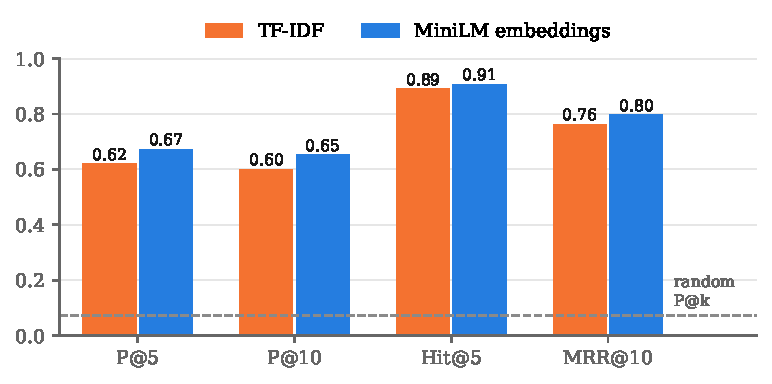
\includegraphics[width=0.75\linewidth]{figures/models.pdf}
  \caption{Test metrics for both candidates. The dashed line is the precision of random ranking.}
  \label{fig:models}
\end{figure}

\begin{figure}[h]
  \centering
  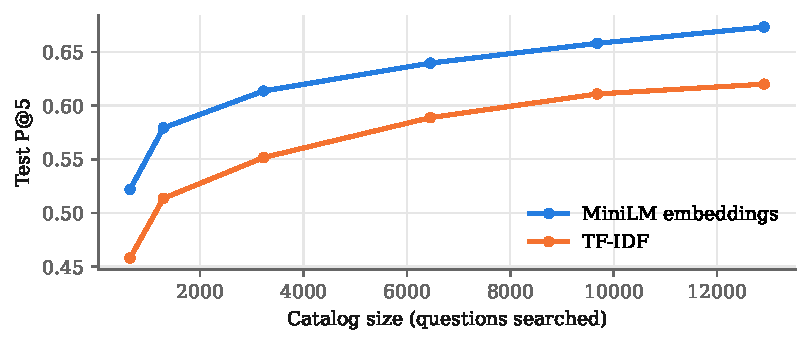
\includegraphics[width=0.75\linewidth]{figures/catalog_size.pdf}
  \caption{Test P@5 as the catalog grows (random subsets of the training set; same 500 queries).}
  \label{fig:catalog}
\end{figure}

The notebook queries with the title and body, but app users type only a title, so we also scored both
models with test titles alone (Table~\ref{tab:title}).

\begin{table}[h]
  \centering\small
  \caption{P@5 with title-only queries, overall and for tags with at least 25 test queries.}
  \label{tab:title}
  \begin{tabular}{l r cc}
    \toprule
    Query subset & $n$ & TF-IDF & MiniLM \\
    \midrule
    All title-only queries         & 500 & 0.589 & 0.653 \\
    \midrule
    \texttt{numpy}                 & 79 & 0.676 & 0.797 \\
    \texttt{matplotlib}            & 72 & 0.764 & 0.836 \\
    \texttt{tensorflow}            & 42 & 0.724 & 0.757 \\
    \texttt{pytorch}               & 34 & 0.635 & 0.741 \\
    \texttt{machine-learning}      & 29 & 0.586 & 0.628 \\
    \texttt{keras}                 & 26 & 0.708 & 0.692 \\
    \texttt{large-language-model}  & 25 & 0.568 & 0.584 \\
    \bottomrule
  \end{tabular}
\end{table}

We chose MiniLM for deployment. It is equal or better on every metric, its P@5 lead of 0.053 is
statistically significant (paired $z = 4.1$), and the lead grows to 0.064 ($z = 5.0$) with title-only
queries, because a short title gives TF-IDF few words to match. It wins on six of the seven most common
tags; the exception is \texttt{keras}, where exact class names such as \texttt{Dense} favour word matching.

MiniLM also needs less data: with a quarter of the catalog it reaches a P@5 of 0.614, close to TF-IDF on
the full catalog (0.620, Figure~\ref{fig:catalog}). For ``how to give a chatbot memory of previous
messages'', TF-IDF's second result is an unrelated SwiftUI chat-interface question; MiniLM's is ``pass
recent history to LLM with current prompt''. Finally, it is
cheaper to run: its index takes 24.8\,MB against 175\,MB for TF-IDF, and a search takes 118\,ms on a
laptop CPU against 176\,ms.
